\documentclass[11pt]{article}
\usepackage[top=1.00in, bottom=1.0in, left=1.1in, right=1.1in]{geometry}
\usepackage{Sweave}
\renewcommand{\baselinestretch}{1.1}
\usepackage{graphicx}
\usepackage{natbib}
\usepackage{amsmath}
\usepackage{gensymb}
\usepackage{parskip}
\usepackage{xcolor}
\usepackage[disable]{todonotes}
\usepackage{xr-hyper}
\usepackage[utf8]{inputenc}
\externaldocument{workingdraft}

\def\labelitemi{--}
\parindent=0pt

\begin{document}

\renewcommand{\refname}{\CHead{}}

% See also: git/grants/crc2023/crc2023app/docs/crc_notes2023more.tex which has some reference notes

\title{Supplement: Why longer seasons with climate change may\\ not increase tree growth}
\author{Team Grephon}
\date{\today}
\maketitle

\renewcommand{\thetable}{S\arabic{table}}
\renewcommand{\thefigure}{S\arabic{figure}}


\section*{Literature review}

We conducted a review to find studies focused on relationships between growing season length and tree wood growth. After reviewing several recent papers \citep{dow2022warm,zohner2023effect}, we searched ISI Web of Science for ``growing season length" AND ``tree ring*" (ALL FIELDS) on 12 April 2023, which returned 33 citations. We next reviewed abstracts and discarded papers that did not mention the relationship between growing season length and growth. We further reviewed all citations within all papers for additionally relevant papers and included them in our review. In total we report on 36 papers after reviewing over 107 potentially relevant papers, after discarding one paper \citep[][which used tree lines as a metric of both growth and growing season length]{bruening2017}. % These ISI methods in outline.tex % grephon_warmingexpts also has some ISI searches, but no date and is focused on warming experiments. 107 is the number in the articles folder. 
% on 31 Oct 2023, I tried ISI (Web of Science Core Collection) for SEARCH tree OR woody (All Fields) and growth (All Fields) and growing season length (All Fields), which returned 886 references. 

Given the large diversity of metrics we found, we did not extract quantitative estimates of growing season length, growth, or their relationship. Instead, we extracted data on location, species, how they measured growing season length, growth, what relationship they found and what internal and external drivers they mentioned (full dataset with more details available on the Knowledge Network for Biocomplexity at publication).

Papers often reported dozens or more statistical tests that were variations of their data, thus we recorded a unique meta-analytic observation (i.e., one row within of data) within each paper (a `study' ID) when papers reported: (1) distinctly different datasets (e.g., a global analyses of observations and a short-term experiment); (2) multiple distinctly different measures of growth (e.g., tree ring width and flux tower) and/or growing season length (e.g., they reported both end of season as budset and end of wood growth through xylogenesis); (3) distinctly different results for growth $\times$  growing season length depending on metric (e.g., using budset for growing season length they find a growth $\times$ growing season length, but using leaf coloring they do not). 

\section*{Towards standardized measurements \& tests}

While our lit review showed that the varying metrics of growth and growing season length can similarly find---or not find---a relationship, we also struggled to make scrape any consistent quantitative estimates---so metrics do matter intensely to helping the field progress. To start the conversation on a standardized set of measurements, we propose:
\begin{enumerate}
\item Ideal measure of growth
\begin{enumerate}
\item Annual increments seem best to me ... no? For long-term forest growth plots, ensuring annual growth measurements paired with phenological measurements would help (most permanent plot data I know of, e.g. FIA and PSP, is collected every 5 years, no phenology). 
\end{enumerate}
\item Ideal measures of wood and vegetative phenology: ideally at the individual level, as satellites cannot differentiate end of season well from herbivory and other factors. Also, given our focus on increment growth, wood phenology is best, but given how hard it is to collect these data we recommend wood phenology people also collect leaf phenology
\begin{enumerate}
\item Xylogenesis folks should measure ....
\item Vegetative: budburst and budset as gold standards for single stages, while photosynthetic measures critical for aligning with satellites etc.. Some of these are time intensive though, so---if you must report more qualitative measures, such as leaf coloring or leaf drop---aim to report several.  
\end{enumerate}
\end{enumerate}

We should also agree on a standardized set of analytical tools. E.g. tree ring analyses --- average away a lot of the interesting things. I<U+2019>m sure there are issues with phenological data, not sure what they are. ... and people should just report direct tests of the relationship so we don't end up with so many `did not measure' answers (Fig. \ref{fig:heatmaps}). And should we recommend tests for lag effects?

\clearpage
\section*{References}
\bibliography{..//bibtex/grephonbib}
\bibliographystyle{/Users/Lizzie/Documents/git/bibtex/styles/besjournals.bst}

\section*{Figures}

\clearpage
\begin{figure}[h!]
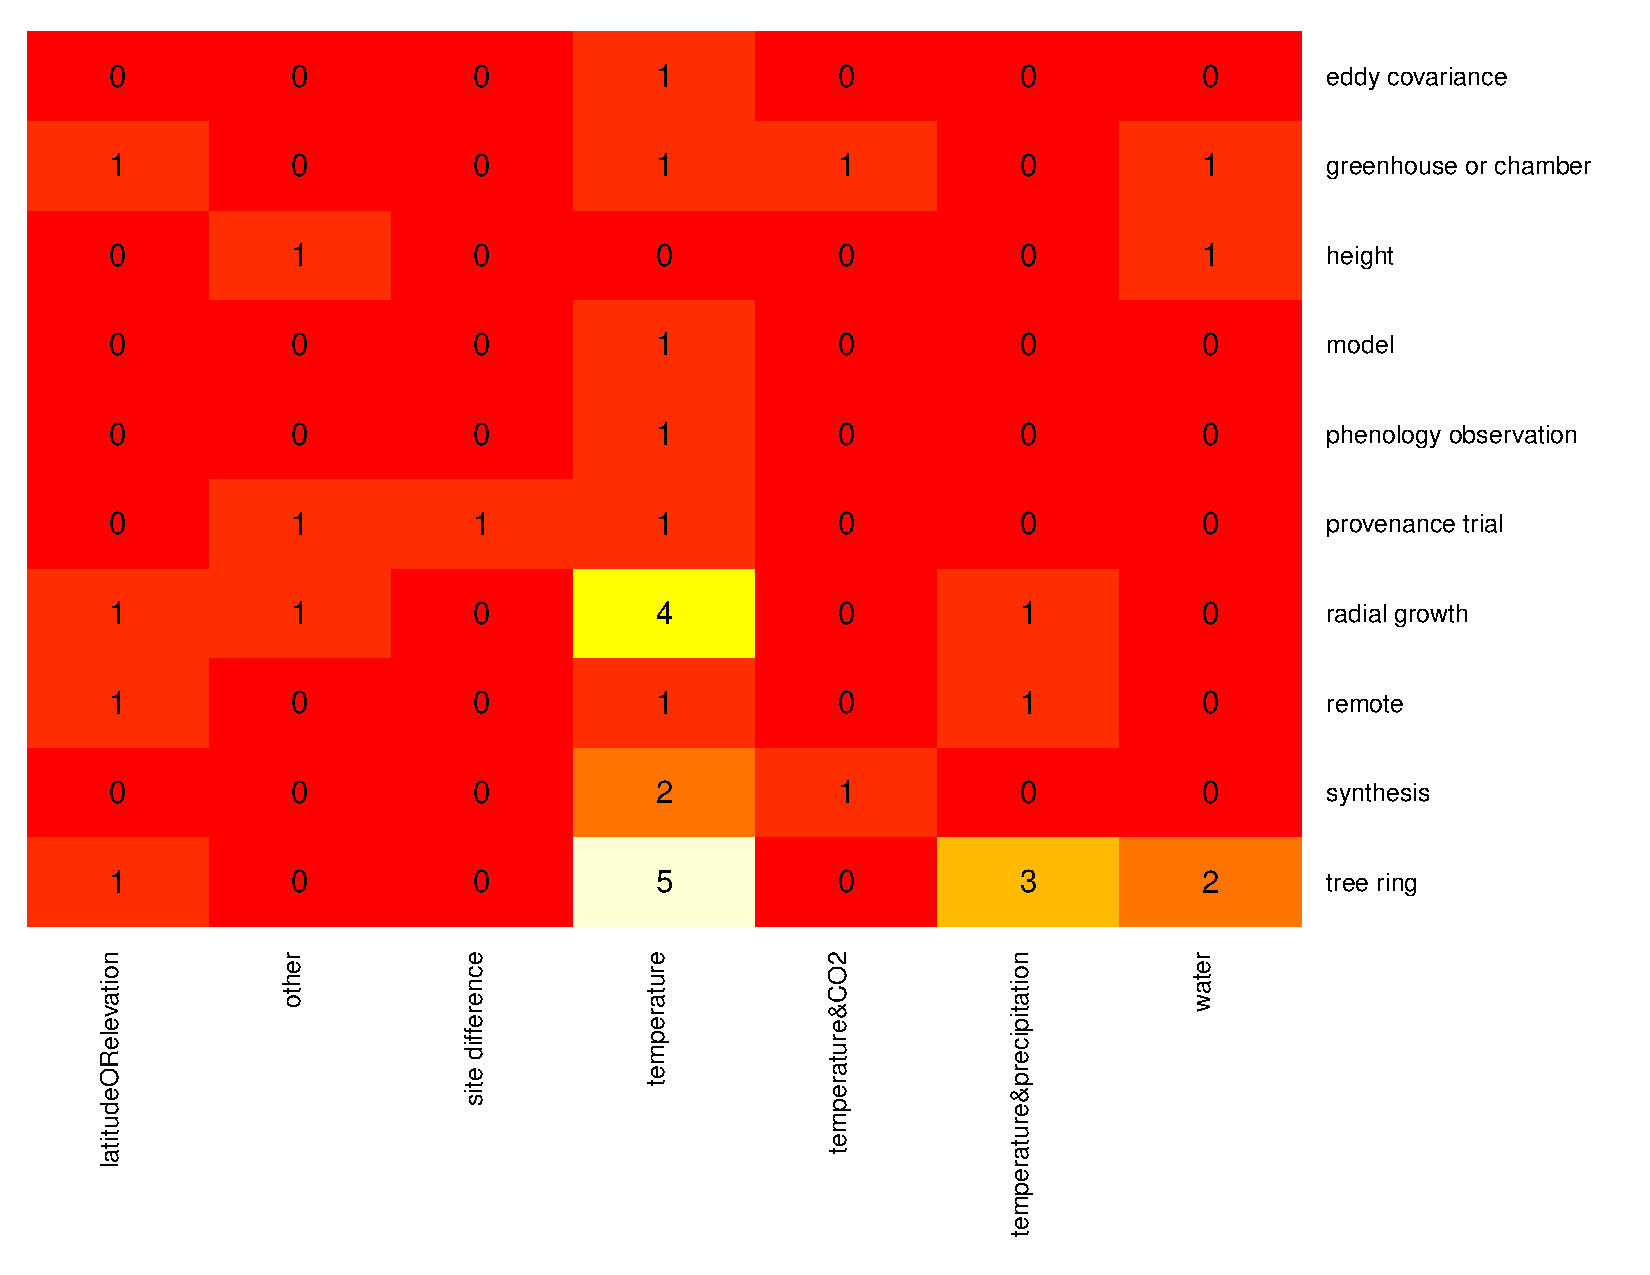
\includegraphics[width=0.8\textwidth]{..//figures/heatmaps/heatmap_extbymethod.pdf}
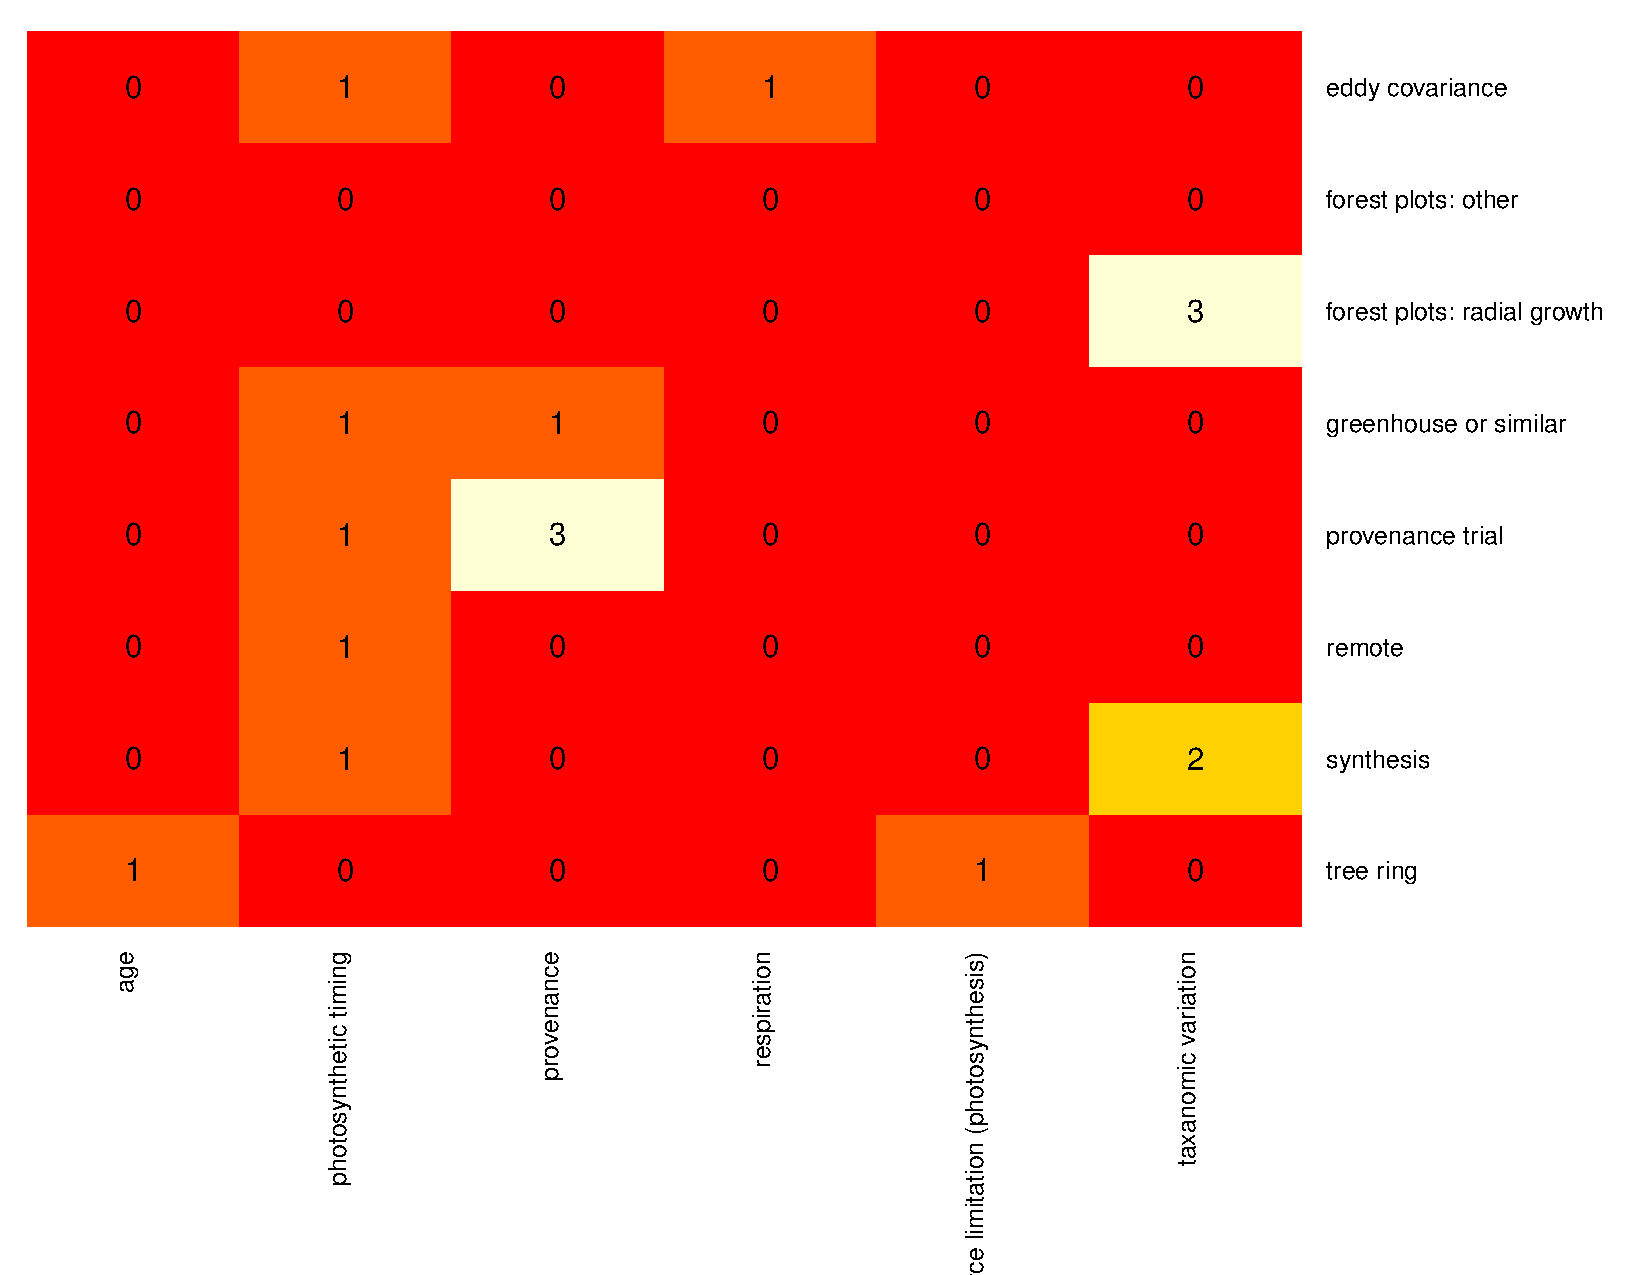
\includegraphics[width=0.8\textwidth]{..//figures/heatmaps/heatmap_endobymethod.pdf}
\caption{Heatmaps from our literature review showing the prevalence of external (top) and internal drivers considered by method (in development).}
\label{fig:heatmapssupp}
\end{figure}



\clearpage
\begin{figure}[h!]
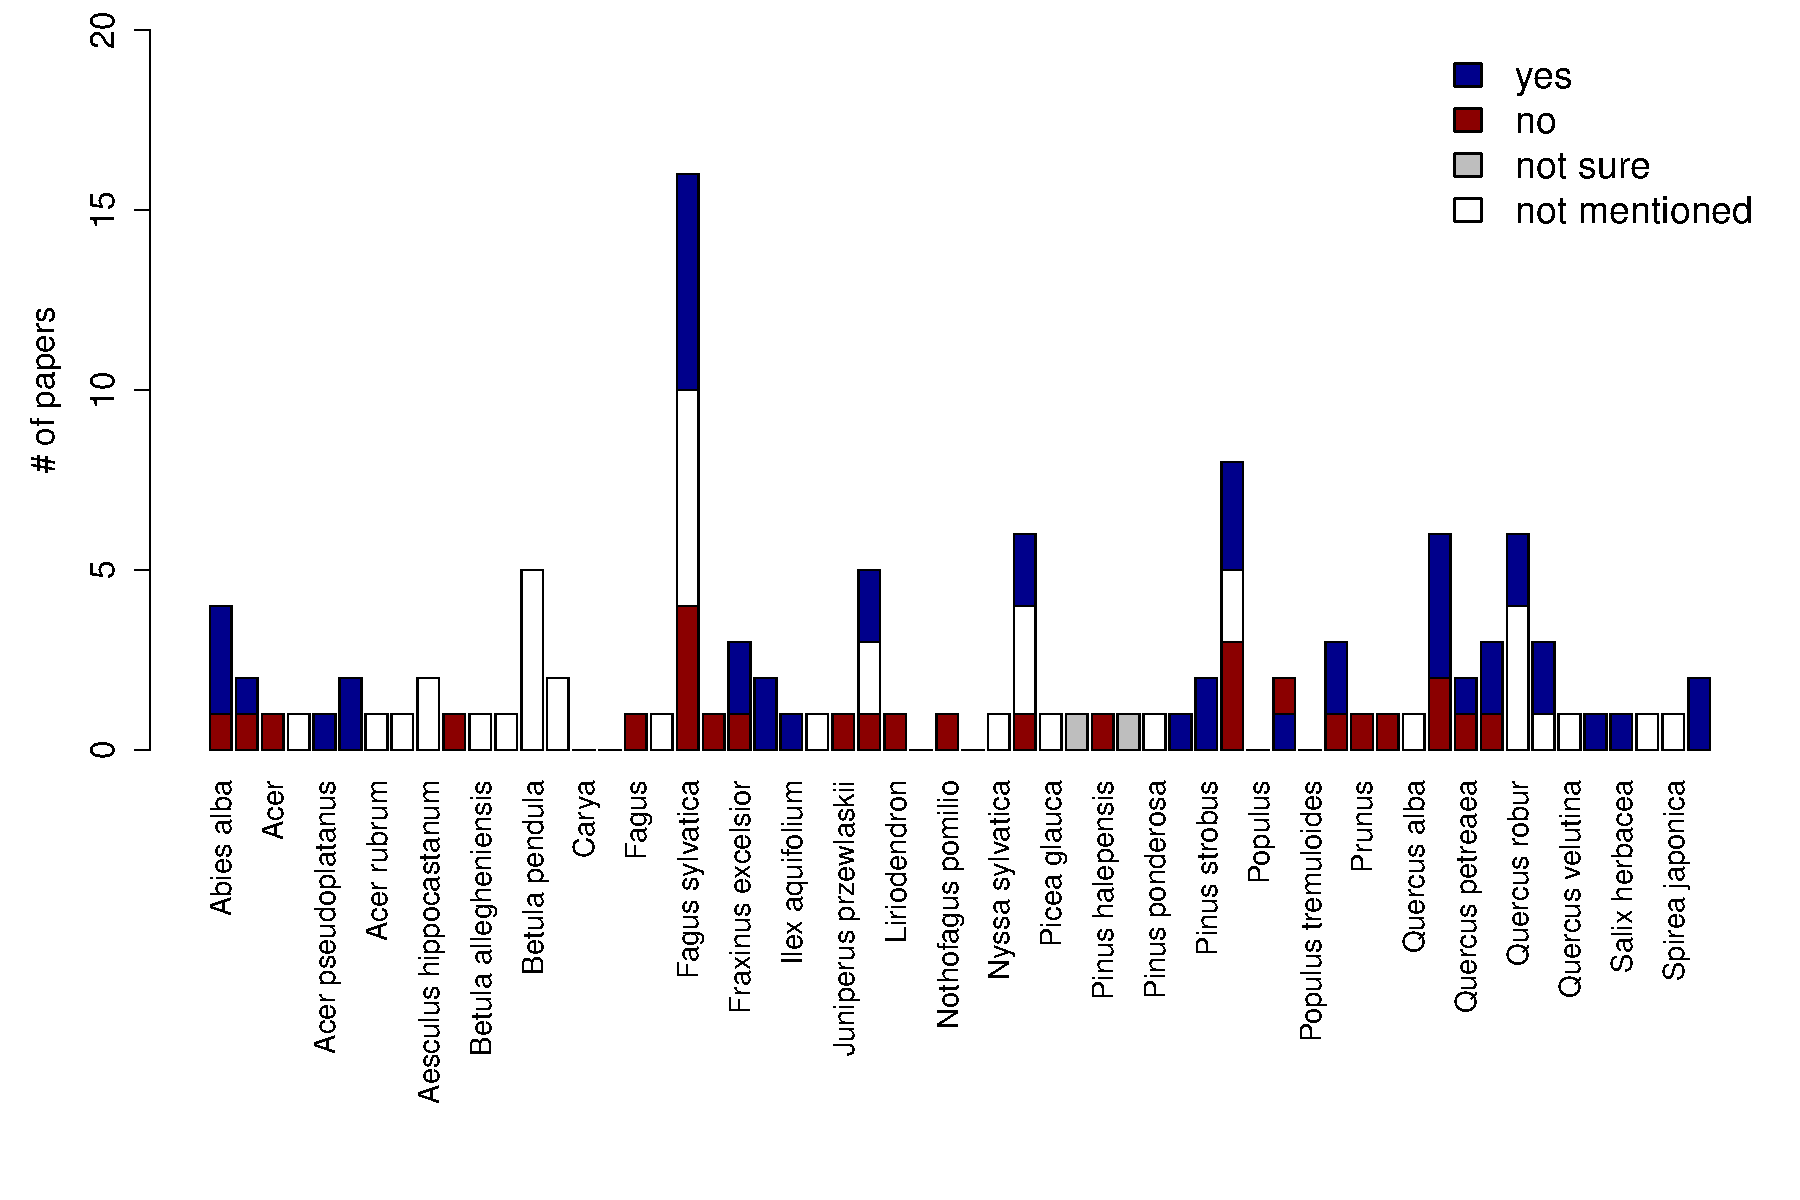
\includegraphics[width=1\textwidth]{..//figures/speciesnums_finds.pdf}
\caption{Results are generally inconsistent across species (in development).}
\label{fig:sppfinds}
\end{figure}


\end{document}
